

\subsubsection{KW49: 06.12.2021 bis 12.12.2021}
\begin{quote}
	\begin{figure}
		\centering
		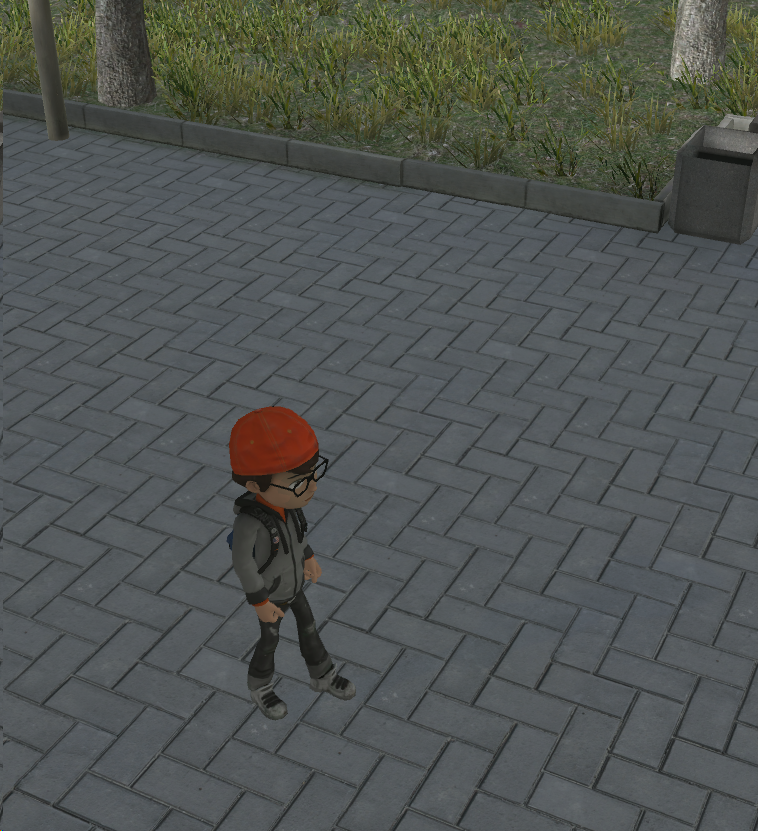
\includegraphics[width=0.7\linewidth]{img/SemihSoenmez_IMG/screenshot002}
		\caption[Charakter]{}
		\label{fig:screenshot002}
	\end{figure}
	
	\subsubsection*{Arbeit in der Schule}
	- Game-Ending Objekt eingefügt: Wenn Hauptcharakter Game-Ending Objekt erreicht wird das Spiel beendet
	- Gegner Gargoyle eingefügt: Wenn Hauptcharakter im PointOfView vom Gargoyle ist, wird Spiel beendet.
	
	
	\subsubsection*{Arbeit außerhalb der Schule}
	- Da unserer Charakter nicht besonders gut ausschaut und in unsere Geschichte nicht hineinpasst, wird stattdessen ein passender Schülercharakter ins Spiel integriert.
	
		- Um dies zu verwirklichen wurde zuerst das fbx Model vom Charakter heruntergeladen.
		
		- Model wurde beim rig auf Humanoid eingestellt und ein neues Avatar wurde erstellt
		
		- funktionierendes Charakter Prefab: Unpack completely
		
		- in Player Armature: Geometry: unser Prefab Model eingefügt
		
		- Sketlon gelöscht
		
		- Avatar von unserem Charakter zugewiesen
	
%	Videos die ich dabei verwendet habe: 
%	https://www.youtube.com/watch?v=jXz5b_9z0Bc

%	https://www.youtube.com/watch?v=0QA2O7juuWQ

%	https://www.youtube.com/watch?v=I_mjYhwSsS8
	
	\subsubsection*{Welche Schwierigkeiten hat es gegeben}
	
\end{quote}

